The previous chapter, Chapter \ref{chap:main}, layed out a holistic framework for \gls{convqa}. This chapter aims to evaluate the applicability of the established system in a real-world scenario. Section \ref{sec:data} describes the available data for the real-world scenario and delves into applied data augmentation techniques. Section \ref{sec:metrics} introduces the metrics used to evaluate the performance of the individual system components, as well as the complete \gls{convqa} system. These metrics are selected based on those used in related work. Section \ref{sec:setup} details the experimental setup, implementation specifics, and provides an implementation framework for similar use cases. Finally, Section \ref{sec:results} presents both quantitative and qualitative results from the experiments.

\section{Data}
\label{sec:data}

To evaluate the proposed system architecture and framework discussed in Chapter \ref{chap:main}, we will implement and assess its performance using the PDFs of the University of Heidelberg's examination regulations (\gls{er}). The university provides these regulations on two separate websites: one in German\footnote{\url{https://www.uni-heidelberg.de/de/studium/studienorganisation/downloadcenter/studien-und-pruefungsordnungen}} and the other in English\footnote{\url{https://www.uni-heidelberg.de/courses/download/examination_rules_regulations.html}}. It's important to note that only the German \gls{er} holds legal authority, and in cases of ambiguity between the English translation and the German original, the German \gls{er} version takes precedence.

Both websites offer structured access to the \gls{er} of nearly all faculties at the University of Heidelberg. However, it's worth mentioning that the German website is regularly updated, while the English version primarily contains outdated \gls{er}. Since there is no centralized source for accessing all English \gls{er}, the decission was made to utilize both the outdated English \gls{er} and the current German \gls{er} for this thesis. This decision aligns with the primary objective of this thesis, which is to demonstrate the \gls{poc} of the introduced framework. Obtaining the latest English \gls{er} of the University of Heidelberg is beyond the scope of this thesis.

As part of the experiments outlined in Section \ref{sec:setup}, the knowledge source of the German \gls{er} will be translated. Additional details on this process can be found in Section \ref{subsec:index}.

The two datasets (German/English) differ in their statistics. Therefore, Figure \ref{fig:er-german-stats} displays the number of documents per faculty regarding the German \gls{er}. Figure \ref{fig:er-english-stats} provides the same statistics for the English \gls{er} dataset. In general, the German dataset consists of 233 individual \gls{er}, while the English dataset contains only 151 individual \gls{er}. As observed, some faculties are overrepresented in both datasets, such as the philosophical faculty. The impact of the document distribution on the system will be discussed in Section \ref{sec:results}.

\begin{figure}
    \centering
    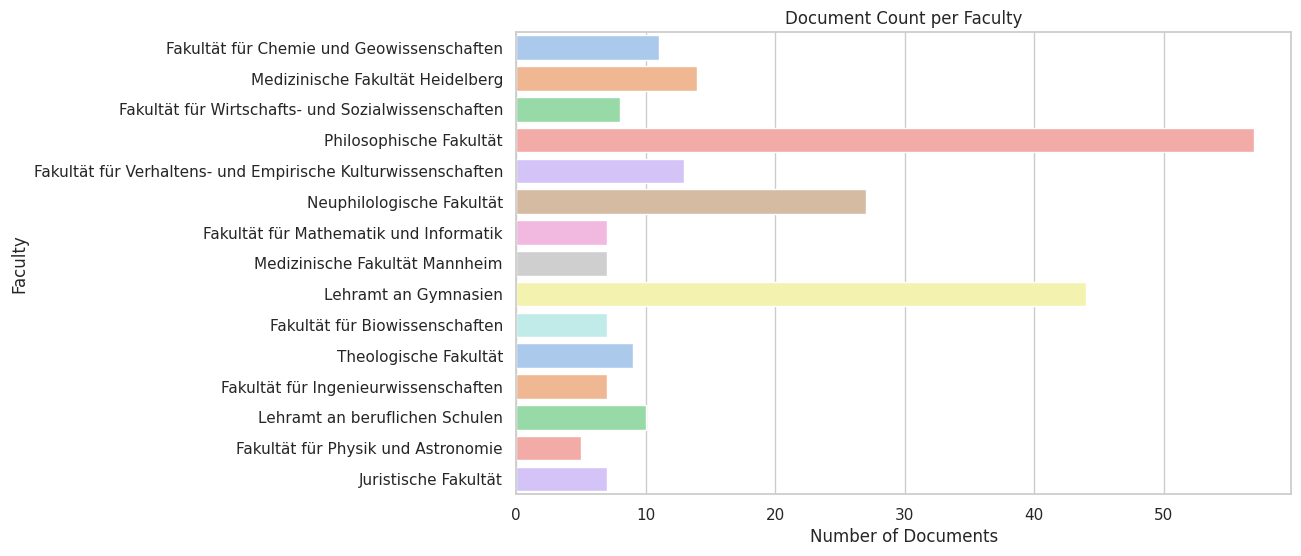
\includegraphics[width=\textwidth]{Grafiken/Statistiken/PO_german_Document Count per Faculty.png}
    \caption{Documents per Faculty of the German \gls{er} Dataset}
    \label{fig:er-german-stats}
\end{figure}

\begin{figure}
    \centering
    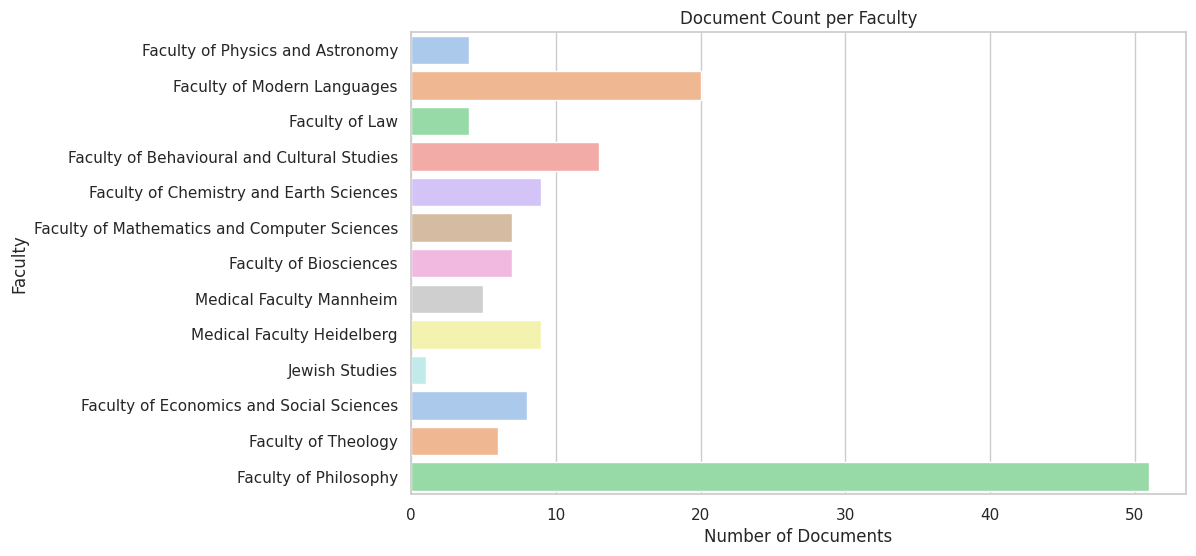
\includegraphics[width=\textwidth]{Grafiken/Statistiken/PO_english_Document Count per Faculty.png}
    \caption{Documents per Faculty of the English \gls{er} Dataset}
    \label{fig:er-english-stats}
\end{figure}

While the previous statistics described the underlying documents of the \gls{poc}, what's even more interesting are the statistics related to the final knowledge source of passages that will be used throughout the \gls{poc}. Details on how these passages have been extracted from the PDFs will be provided in Section \ref{subsec:index}. In this section, we will focus on the statistical analysis.

\begin{figure}
    \centering
    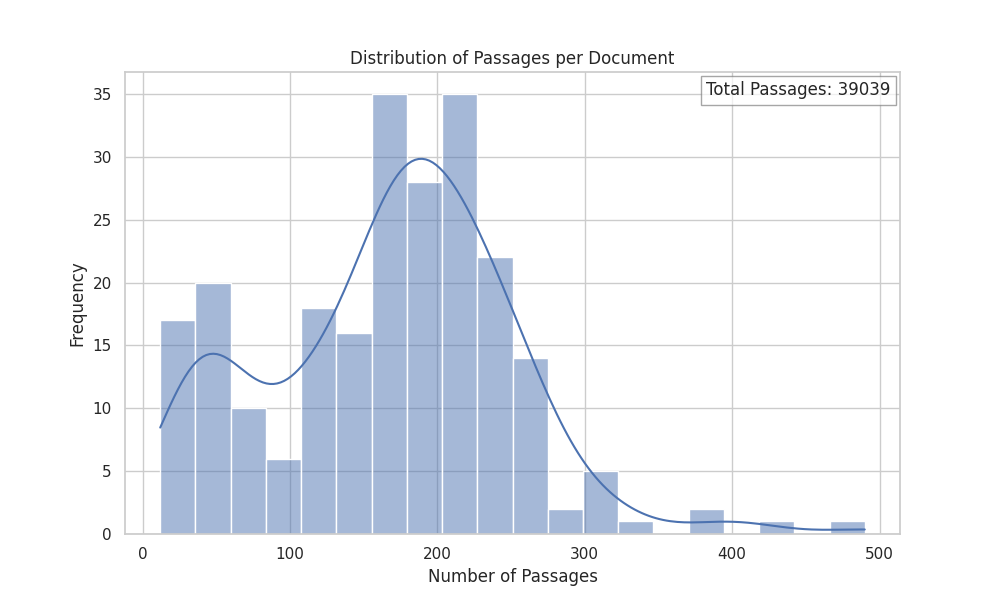
\includegraphics[width=\textwidth]{Grafiken/Statistiken/IndexGerman_Passages_Distribution.png}
    \caption{Passages per Document of the German \gls{er} Dataset}
    \label{fig:er-german-passage-document}
\end{figure}

\begin{figure}
    \centering
    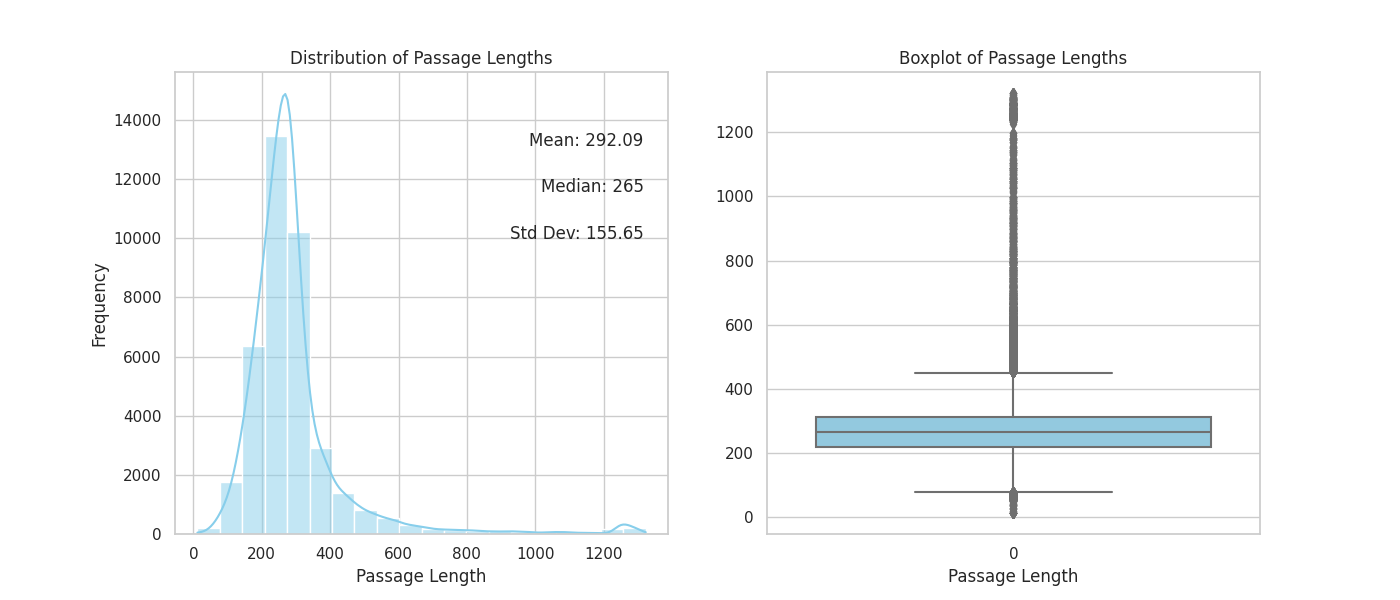
\includegraphics[width=\textwidth]{Grafiken/Statistiken/IndexGerman_Passage_Length_Statistics.png}
    \caption{Passage Length Distribution of the German \gls{er} Dataset}
    \label{fig:er-german-passage-length}
\end{figure}
Figure \ref{fig:er-german-passage-document} illustrates the distribution of passages across documents in the German dataset, offering insights into the diverse influence that documents can have on the knowledge source in terms of the number of passages. These differences in passages are mainly due to variations in the length of the examination regulations (\gls{er}). The total number of passages in the German dataset is 39,039, resulting in an average of 167.55 passages per document. In comparison, the English dataset has an average of 212.94 passages per document. The statistics for the translated dataset are similar to those of the German dataset. An apparent difference between these two datasets is that the distribution of German passages per document exhibits a slight camel-like shape with a local maximum, while the English distribution follows a clear Gaussian pattern. However, these distribution differences are not further evaluated, as we assume that they do not significantly impact the system's quality.

Figure \ref{fig:er-english-passage-document} presents the same statistics for the English dataset. As observed, the English knowledge source is smaller (31,659 vs. 38,642) than the German one, which is expected given that the English dataset contains only 151 \gls{er} compared to the 233 German \gls{er}. Still, the average number of passages per document is higher in the English dataset, as mentioned earlier. The total number of passages in the knowledge source indicates a highly closed-domain scenario. For comparison, MS MARCO \cite{bajaj2016ms}, an often-used dataset for open-domain \gls{qa}, has a knowledge source comprising 3.2 million passages, with an average length of 442 characters and passages ranging from 19 to 1,167 characters.

Figure \ref{fig:er-german-passage-length} depicts the distribution of passage lengths in the German dataset. It's evident that the majority of passages fall within the range of 200 to 350 characters. The same statistics for the English dataset are presented in Figure \ref{fig:er-english-passage-length}. As observed, they are quite similar. The shortest passage is 5 characters, as we applied a lower filter to the extracted passages. The longest passages are 1,300 characters long, also subjected to filtering. Considering statistics such as standard deviation, mean, and median, the English and German datasets do not significantly differ in terms of passage length.


\begin{figure}
    \centering
    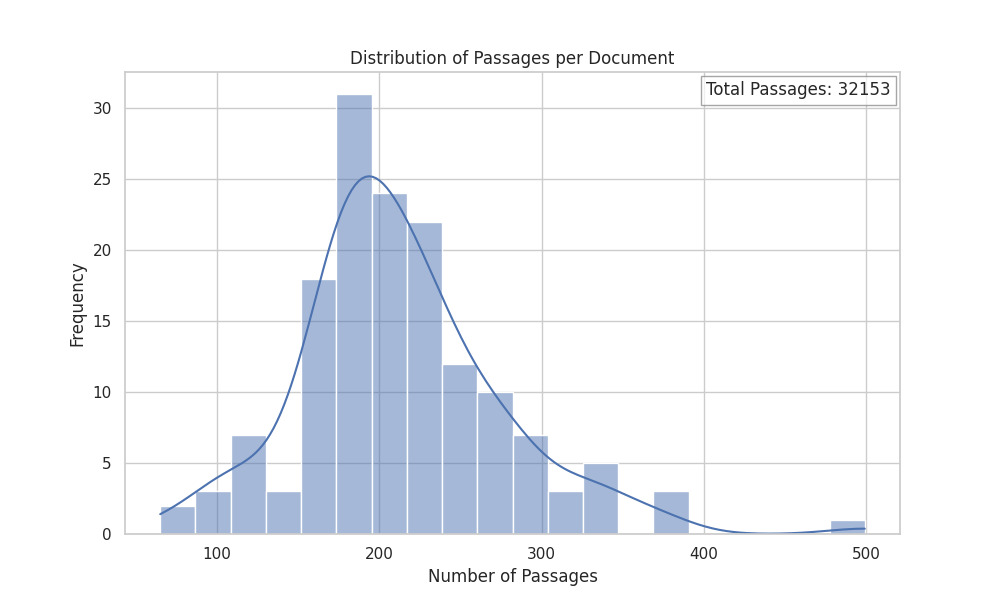
\includegraphics[width=\textwidth]{Grafiken/Statistiken/IndexEnglish_Passages_Distribution.png}
    \caption{Passages per Document of the English \gls{er} Dataset}
    \label{fig:er-english-passage-document}
\end{figure}

\begin{figure}
    \centering
    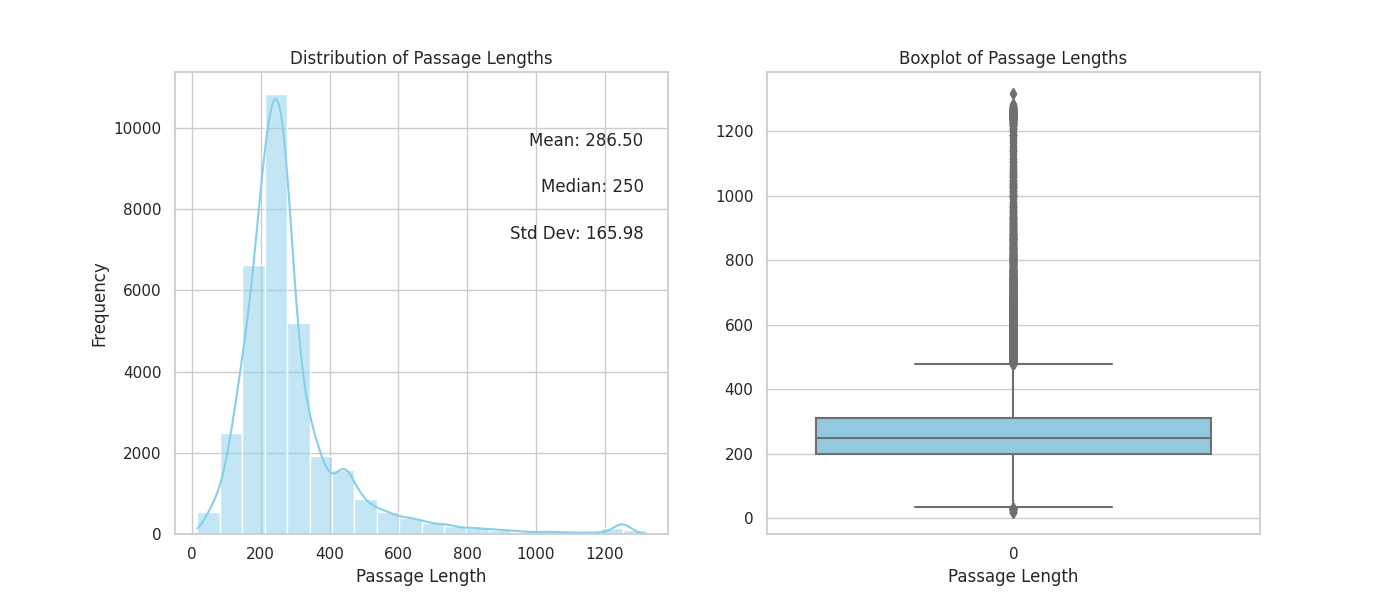
\includegraphics[width=\textwidth]{Grafiken/Statistiken/IndexEnglish_Passage_Length_Statistics.png}
    \caption{Passage Length Distribution of the English \gls{er} Dataset}
    \label{fig:er-english-passage-length}
\end{figure}


\section{Evaluation Metrics}
\label{sec:metrics}

When it comes to Evaluation Metrics, it's important to differentiate between the components or models being evaluated. For the evaluation, we will categorize the evaluation scopes as follows:

\begin{enumerate}
    \item Retrieval
    \item Reader
    \item Conversational Question Answering
\end{enumerate}

Evaluating the \gls{cqu} component is only possible with high quality human supervised datasets, therefore for the performance of the \gls{cqu} section \ref{subsec:cqu-impl} refers to previously by other works performed benchmarks of the used zero-shot models. The exact metrics and paradigms for each individual evaluation will be discussed in the following sections.

\subsection{Retrieval Evaluation}
\label{subsec:retrieval-eval}

Evaluating a Retriever largely depends on the use-case and the evaluation data available. Since the data introduced in Section \ref{sec:data} lacks a supervised dataset for $(question,\allowbreak passages)$ pairs, we will evaluate it using the synthetic dataset created, as also established in Section \ref{sec:data}. This dataset consists of $(question, passages)$ pairs, where for every question, there is an exact matching passage. Therefore, this dataset is essentially a binary task, where a passage is either the correct one or not. An alternative approach would be a graded relevance task, where each passage has a certain relevance score in relation to the question. However, for our use-case, we opted for the simpler metrics \gls{hr}@k and \gls{mrr}, instead of the Normalized Cumulative Gain (NDCG) used in benchmarks like BEIR \cite{thakur_beir_2021}. We chose these metrics because it's crucial for our system to retrieve the correct passage, and we don't have a relevance score for every passage in relation to every question.

Given a pair of $(q,\hat{p})$, where $\hat{p}$ corresponds to the correct passage and $\forall q, \exists ! \hat{p} \in P$ and a retriever model $p_\eta(p|q) = \text{Score}(q,p)$ (as defined in Definition \ref{def:retrieval}) that assigns a score to every passage $p \in P$ in relation to the question $q$ is used. We can rank all passages based on their relevance to $q$. Each passage receives a rank $r_q,p$ based on its score in relation to $q$. These passages are then ranked in descending order of $r_q,p$, and the top $k$ passages are added to the retrieved set $R_q$.

\begin{itemize}
    \item \textbf{\gls{hr}@k} This metric calculates the proportion of questions for which the correct passage is retrieved within the top $k$ retrieved passages.
    \begin{equation}
        \text{HR@k} = \frac{1}{|Q|} \sum_{q \in Q} 
        \begin{cases}
            1 & \text{if } \hat{p}_q \in R_{q,k} \\
            0 & \text{otherwise}
        \end{cases}
        \in [0,1]
    \end{equation}
    The \gls{hr}@k is a straightforward metric that provides a value between 0 and 1, with a higher value indicating the percentage of cases where the correct passage was retrieved within the top $k$ passages.
    \item \textbf{\gls{mrr}} This metric computes the mean reciprocal rank of the correct passage. It is similar to \gls{hr}@k but considers the position of the correct passage $\hat{p}q$ within the ranking $R_q$.
    \begin{equation}
        \text{MRR} = \frac{1}{|Q|} \sum_{q \in Q} \frac{1}{r_{q,\hat{p}_q}} \in [0,1]
    \end{equation}
    In an ideal system, the \gls{mrr} would be 1, indicating that the correct passage is always retrieved in the first position ($r_{q,\hat{p}} = 1$) for all $q \in Q$.
\end{itemize}

\subsection{Reader Evaluation}
\label{subsec:answer-generation-eval}

Evaluating the task of answer generation, particularly the \gls{mrc} aspect of the reader component, presents challenges similar to those discussed for the retrieval task evaluation in Section \ref{subsec:retrieval-eval}. For automatic and manual evaluation, we will utilize the synthetic dataset generated in Section \ref{sec:data}. This dataset comprises triples of $(\text{question}, \text{passages}, \text{answer})$, where \textit{answer} refers to a gold answer that has been syntactically generated.

In the context of a triple $(q, \hat{p}, \hat{a})$, where $\hat{p}$ corresponds to the correct passage and $\hat{a}$ corresponds to the correct answer in relation to a question $q$, we employ a reader model $p_\theta(a' \, | \, q, \hat{p}) := \hat{a}$ (as defined in Definition \ref{def:generation}) to predict the answer $\hat{a}$ given the question $q$ and the passage $\hat{p}$. The predicted answer $a'$ is then evaluated using the following metrics:

\begin{itemize}
    \item \textbf{BLUE-1:} This precision-oriented metric compares the occurrence of unigrams (words $w \in \hat{a}$) in the predicted answer $a'$ and the gold answer $\hat{a}$.
    \begin{equation}
        \text{BLUE-1} = \frac{\sum_{w \in a'} \min(\text{count}_{a'}(w), \text{count}_{\hat{a}}(w))}{\sum_{w \in a'} \text{count}_{a'}(w)} \in [0,1]
    \end{equation}
    Here, $\text{count}_{a'}(w)$ represents the number of occurrences of the word $w$ in the predicted answer $a'$. \gls{bleu} is particularly useful for evaluating extractive questions \cite{papineni_bleu_2002}.

    \item \textbf{ROUGE-L:} This recall-oriented metric, especially \gls{rogue}-L, compares the longest common subsequence ($LCS$) between the predicted answer $a'$ and the gold answer $\hat{a}$.
    \begin{align}
        R_{LCS} &= \frac{LCS(\hat{a}, a')}{|\hat{a}|} \\
        P_{LCS} &= \frac{LCS(\hat{a}, a')}{|a'|} \\
        \text{ROUGE-L} &= \frac{(1+\beta^2)R_{LCS}P_{LCS}}{R_{LCS}+\beta^2P_{LCS}} \in [0,1]
    \end{align}
    Here, $\beta$ is a parameter to balance between precision and recall. Rouge operates similarly to \gls{bleu} but focuses on lexical matching \cite{lin_rouge_2004}.

    \item \textbf{F1-BERTscore}: BERTscore is a \gls{s2s}-model-based evaluation metric for comparing two text fragments: $x$, which is the reference, and $\hat{x}$, which is the prediction. In this context, the predicted answer $a'$ is compared to the gold answer $\hat{a}$. Essentially, the score between two tokens, $a'_i$ and $\hat{a}_i$, is calculated as the inner product of their respective BERT embeddings: $\text{BERT}(a'_i)^T\text{BERT}(\hat{a}_i)$. For simplicity, we'll use the  $\text{BERT}(a'_i) \rightarrow a'_i$ in the following equations. The final scores of F1-BERTscore are weighted by the inverse document frequency (idf) of each word-piece token:

    \begin{align}
        P_{BERT} &= \frac{\sum_{a'_j\in a'} \text{idf}(a') \max_{\hat{a}_i \in \hat{a}} (\hat{a}_i^T a'_j)}{\sum_{a'_j\in a'} \text{idf}(a')} \\
        R_{BERT} &= \frac{\sum_{\hat{a}_i \in \hat{a}} \text{idf}(\hat{a}_i) \max_{a'_j \in a'} (\hat{a}_i^T a'_j)}{\sum_{\hat{a}_i \in \hat{a}} \text{idf}(\hat{a}_i)} \\
        F1_{BERT} &= \frac{2P_{BERT}R_{BERT}}{P_{BERT}+R_{BERT}}
    \end{align}
    
    The advantage of F1-BERTscore lies in its reliance on semantic matching between the gold answer $\hat{a}$ and the predicted answer $a'$ rather than mere lexical matching \cite{zhang_bertscore_2020}.
    

    \item \textbf{Accuracy} This metric calculates the proportion of questions for which the predicted answer $a'$ matches the gold answer $\hat{a}$. 
    \begin{equation}
        \text{Accuracy} = \frac{1}{|Q|} \sum_{q \in Q} 
        \begin{cases}
            1 & \text{if } a' = \hat{a} \\
            0 & \text{otherwise}
        \end{cases}
        \in [0,1]
    \end{equation}
    This metric is useful for evaluating question, answer realtions, where there is only one correct answer. In order to define if an answer is correct or not, the following approaches will be used:
    \begin{itemize}
        \item \textbf{LLM-based:} A \gls{llm} can be prompted to determine a binary value (0 or 1) indicating whether the underlying message of $a'$ and $\hat{a}$ matches. The prompt used is based on the work of \cite{kamalloo_evaluating_2023}:
        \begin{quote}
            \texttt{Question:} q \\
            \texttt{Gold Answer:} $\hat{a}$ \\
            \texttt{Predicted Answer:} a' \\
            \texttt{Is the predicted answer correct?} Yes/No
        \end{quote}
        This appraoch is especially useful for evaluating generative questions, as it allows for semantic matching.
        \item \textbf{Human-based:} A human evaluator is asked to assign a binary value of 0 or 1 to indicate whether there is a match in the underlying message of $a'$ and $\hat{a}$. 1 if the answer $a'$ covers the information from $\hat{a}$, and 0 if it does not. The evaluator is provided with the question $q$, the important passage $\hat{p}$, the gold answer $\hat{a}$, and the generated answer $a'$. This approach is particularly useful for evaluating generative questions and closely resembles real-world applications. For this thesis two evaluaters will receive the same 100 randomly sampled answers and will be asked to assign a binary value to each answer. The inter-rater agreement will be calculated using Cohen's Kappa \cite{cohen_coefficient_1960}. 
    \end{itemize}
\end{itemize}
    
\subsection{Conversational Question Answering Evaluation}
\label{subsec:convqa-eval}

The most challenging aspect of evaluation within the context of the system developed here is assessing \gls{convqa} as a holistic system. Instead of presenting evaluation metrics in this section, we will explore the approaches for evaluating \gls{convqa}, and as final metrics, we will use those introduced in Sections \ref{subsec:answer-generation-eval} and \ref{subsec:retrieval-eval}. Generally, two approaches can be considered: 

The first approach, known as \textbf{Manual Human Evaluation (\gls{mahueval})}, operates as follows:

\begin{enumerate}
    \item A human evaluator initiates a conversation with a question, either based on their own intuition or using provided questions from the supervised dataset. Evaluators are encouraged to pose context-dependent questions.
    \item The evaluator continues the conversation, asking follow-up questions or engaging in a general discussion with the \gls{convqa}-System for 8-10 turns.
    \item After the conversation, the evaluator has access to the retrieved passages $p$ for each turn and all other passages $P$ in the index. The evaluator assesses the answer provided by the system and the relevance of the retrieved passages $p$. They are required to provide the following information:
        \begin{itemize}
            \item \textit{Question Intent:} The evaluator specifies the intent of the question, which can be categorized as either \textit{extractive}, \textit{abstractive}, or \textit{boolean}.
            \item \textit{Answer:} The evaluator assigns a binary value (0 or 1) to the system's answer. A score of 1 indicates a correct answer, while 0 represents an incorrect answer.
            \item \textit{Passage:} The evaluator assigns a binary value (0 or 1) to the relevance of the retrieved passages $p$. A score of 1 indicates that the passages are relevant for generating the correct answer, while 0 indicates irrelevance.
        \end{itemize}
    \item Based on the provided scores, metrics for the retriever and reader will be calculated for each turn, the entire conversation history, and the entire dataset. \textit{Accuracy} will be computed for answers, and \textit{HR@k} will be computed for passages. All results will be grouped by turn, enabling deeper insights into the performance and errors of the system.
\end{enumerate}

To mitigate bias, human manual evaluations are conducted by two different evaluators. Each evaluator conducts 10 conversations with the system in the first round. In the second round, the evaluators initiate conversations with the first question from the 10 conversations of the other evaluator. This results in a total of 40 conversations and, ideally, 20 overlapping conversations that can be used to calculate inter-rater agreement \cite{cohen_coefficient_1960}.

The second approach, \textbf{\gls{auev}}, operates as follows. In this approach, a synthetic dataset is provided, consisting of lists of triples $(q, \hat{p}, \hat{a})$, where each triple corresponds to one turn, and a list represents a conversation history $h \in H$:

\begin{enumerate}
    \item Initially, the system is presented with the first question $q_1$ from the conversation history. The response $a'_1$ is evaluated using the \textit{F1-BERTscore} in comparison to the gold answer $\hat{a}$ of the history $h$. This score is computed for each turn, assessing the system's response against the gold answer for that turn.
    \item Subsequently, to mitigate the impact of an incorrect system response on the ongoing conversation, the following question (e.g., $q_2$) is augmented with the gold answer $\hat{a}_1$. This augmentation helps address missing information or coreference problems caused by an erroneous response. This method, originally introduced by Li et al. \cite{li_ditch_2022}, improves the automatic evaluation of \gls{convqa} systems. The model used to resolve the relationship between the gold answer and the question is the standard CQU model. Additionally, within the \gls{convqa} history, the answer $a'_1$ is replaced by the gold answer $\hat{a}_1$ for the CQU unit.
    \item After enhancing the question, the system is tasked with generating a response $a'_2$ to the augmented question $q'_2$. Once again, the response $a'_2$ is evaluated using the \textit{F1-BERTscore} against the gold answer $\hat{a}_2$ from the history $h$.
    \item Steps (2) and (3) are repeated until the end of the conversation history $h$.
    \item All scores will be groupable by turn depth, enabling deeper insights into the performance and errors of the system.
\end{enumerate}

Both \gls{mahueval} and \gls{auev} will be employed to evaluate the \gls{convqa} system, and the results will be reported separately.

\section{Experimental Setup and Implementation}
\label{sec:setup}

This section outlines the experimental setup and provides details on the implementation of the System Architecture and Framework introduced in Chapter \ref{chap:main}. First and foremost, we apply the theoretically outlined model ($M$) to create an implementation decision map. Figure \ref{fig:extract-pipeline-implementation-grid} illustrates a decision tree showcasing the possible implementations of the \textit{Extract} pipeline. Figure \ref{fig:all-components-conrag-grid} displays the main components, namely the \textit{Retriever}, \textit{Reader}, and \textit{\gls{cqu}}, in a similar decision matrix, where each column represents a decision to be made during implementation. Opting not to make a decision is also a valid choice. Developing an implementation can then be easily achieved using a decision tree, as shown in Figure \ref{fig:example-implementation-tree}. For the implementation and benchmarking, ressources of the BwUniCluster\footnote{\url{https://wiki.bwhpc.de/e/BwUniCluster2.0}} have been used.

\begin{figure}
    \centering
    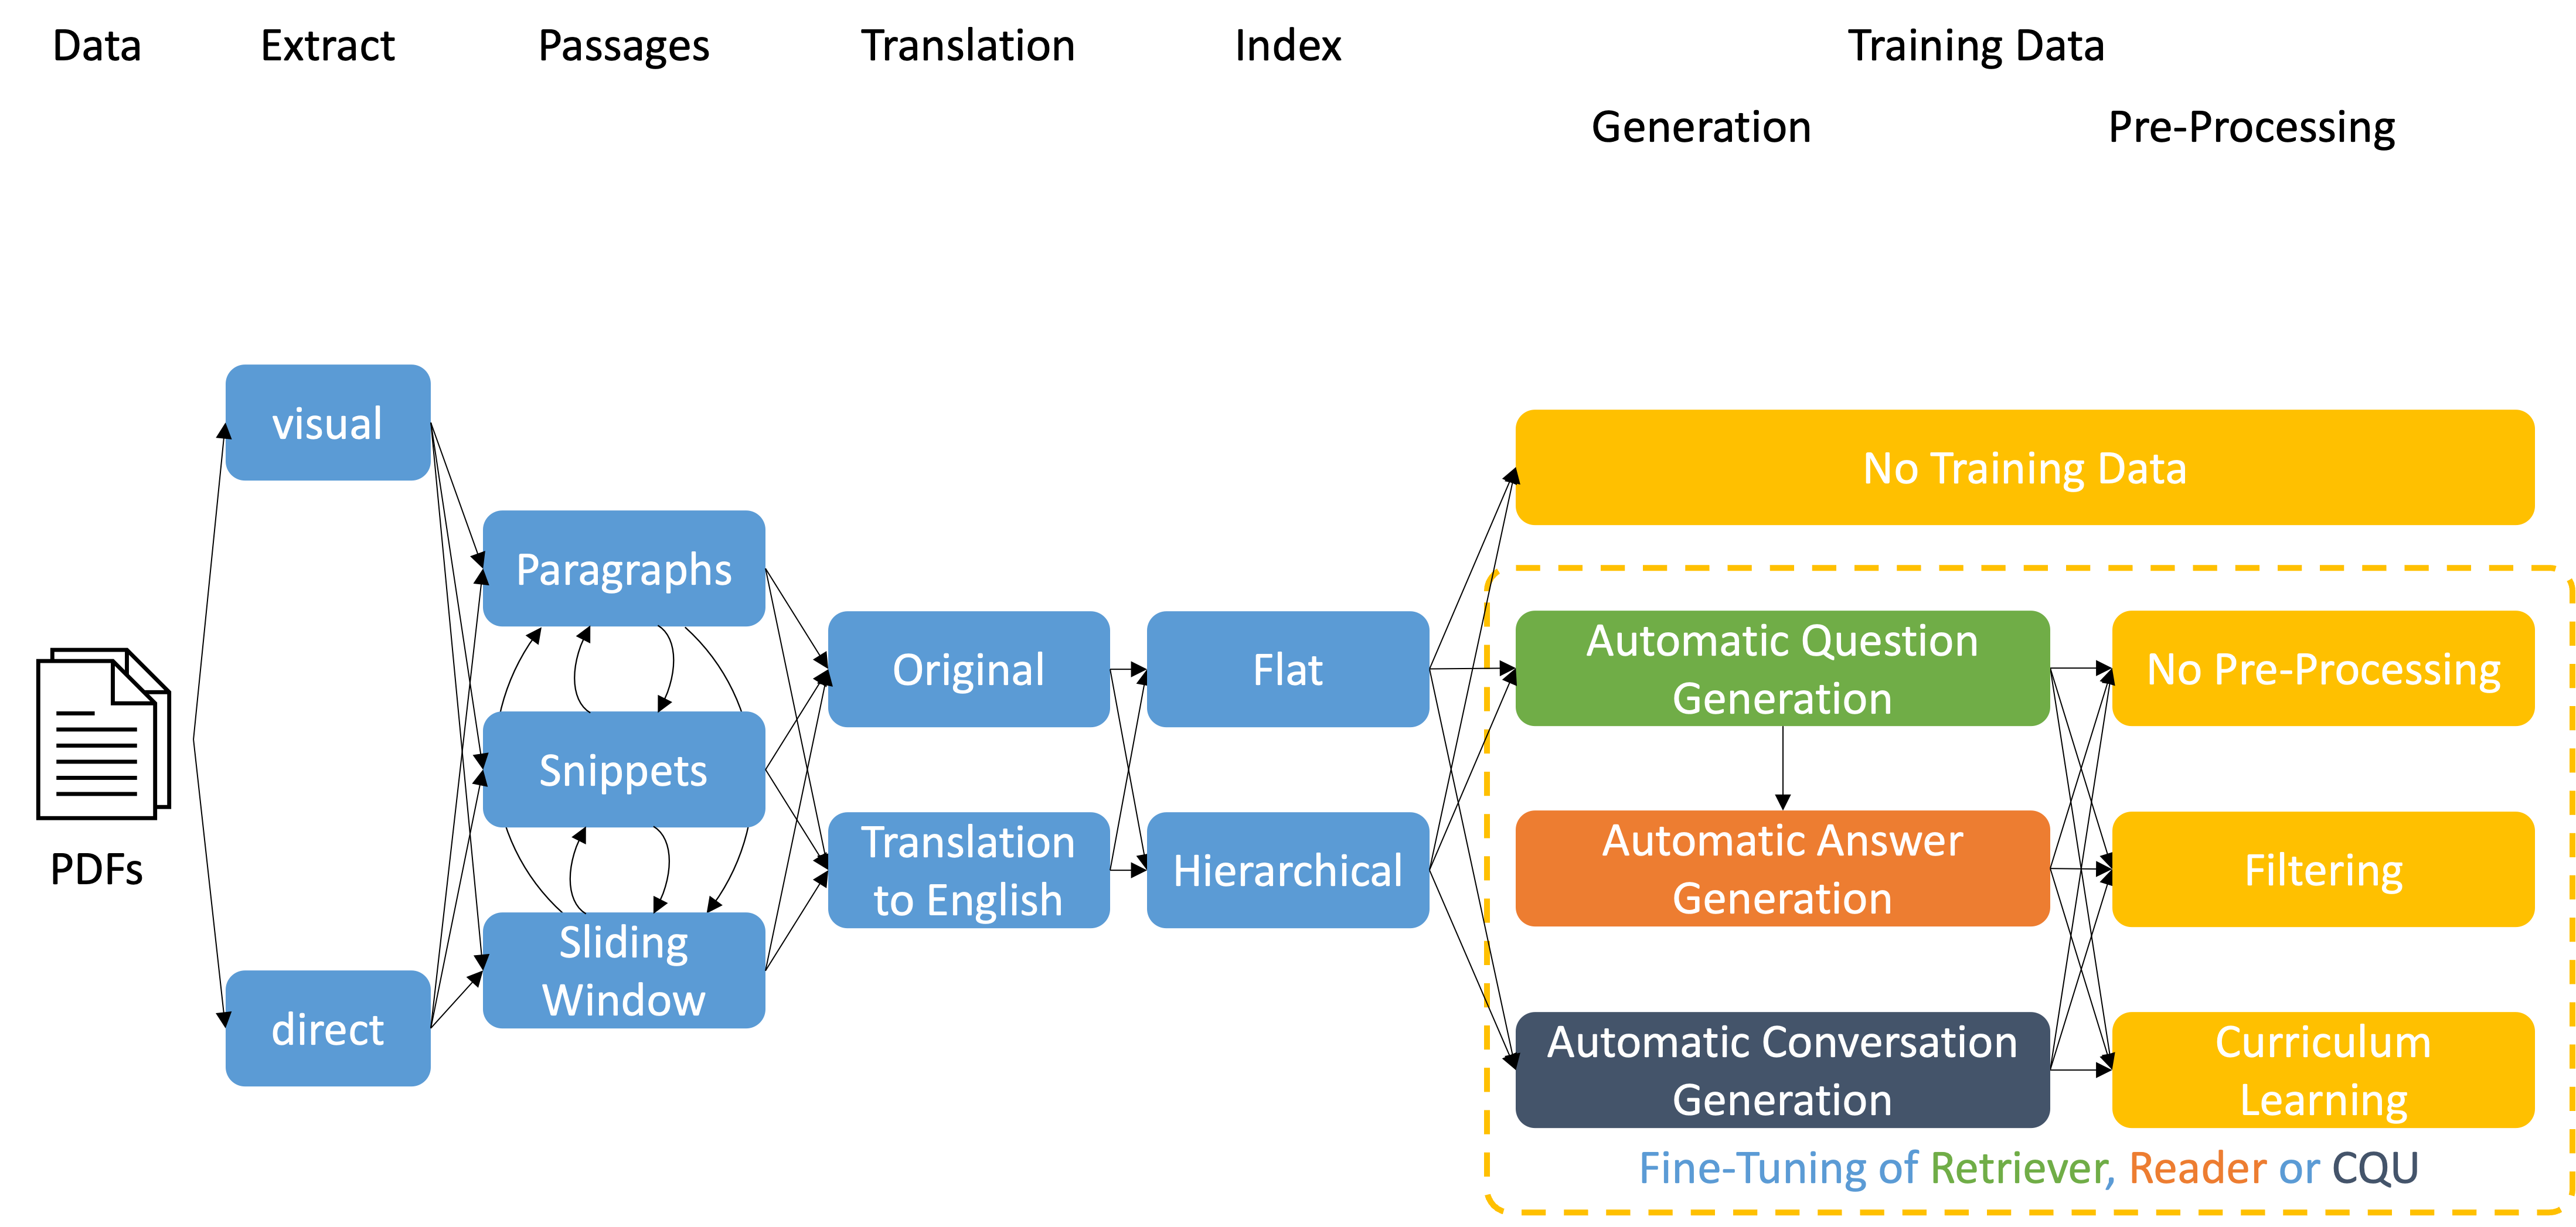
\includegraphics[width=\textwidth]{Grafiken/extract_pipeline.png}
    \caption{Possible Implementations of the Extract Pipeline}
    \label{fig:extract-pipeline-implementation-grid}
\end{figure}

\begin{figure}
    \centering
    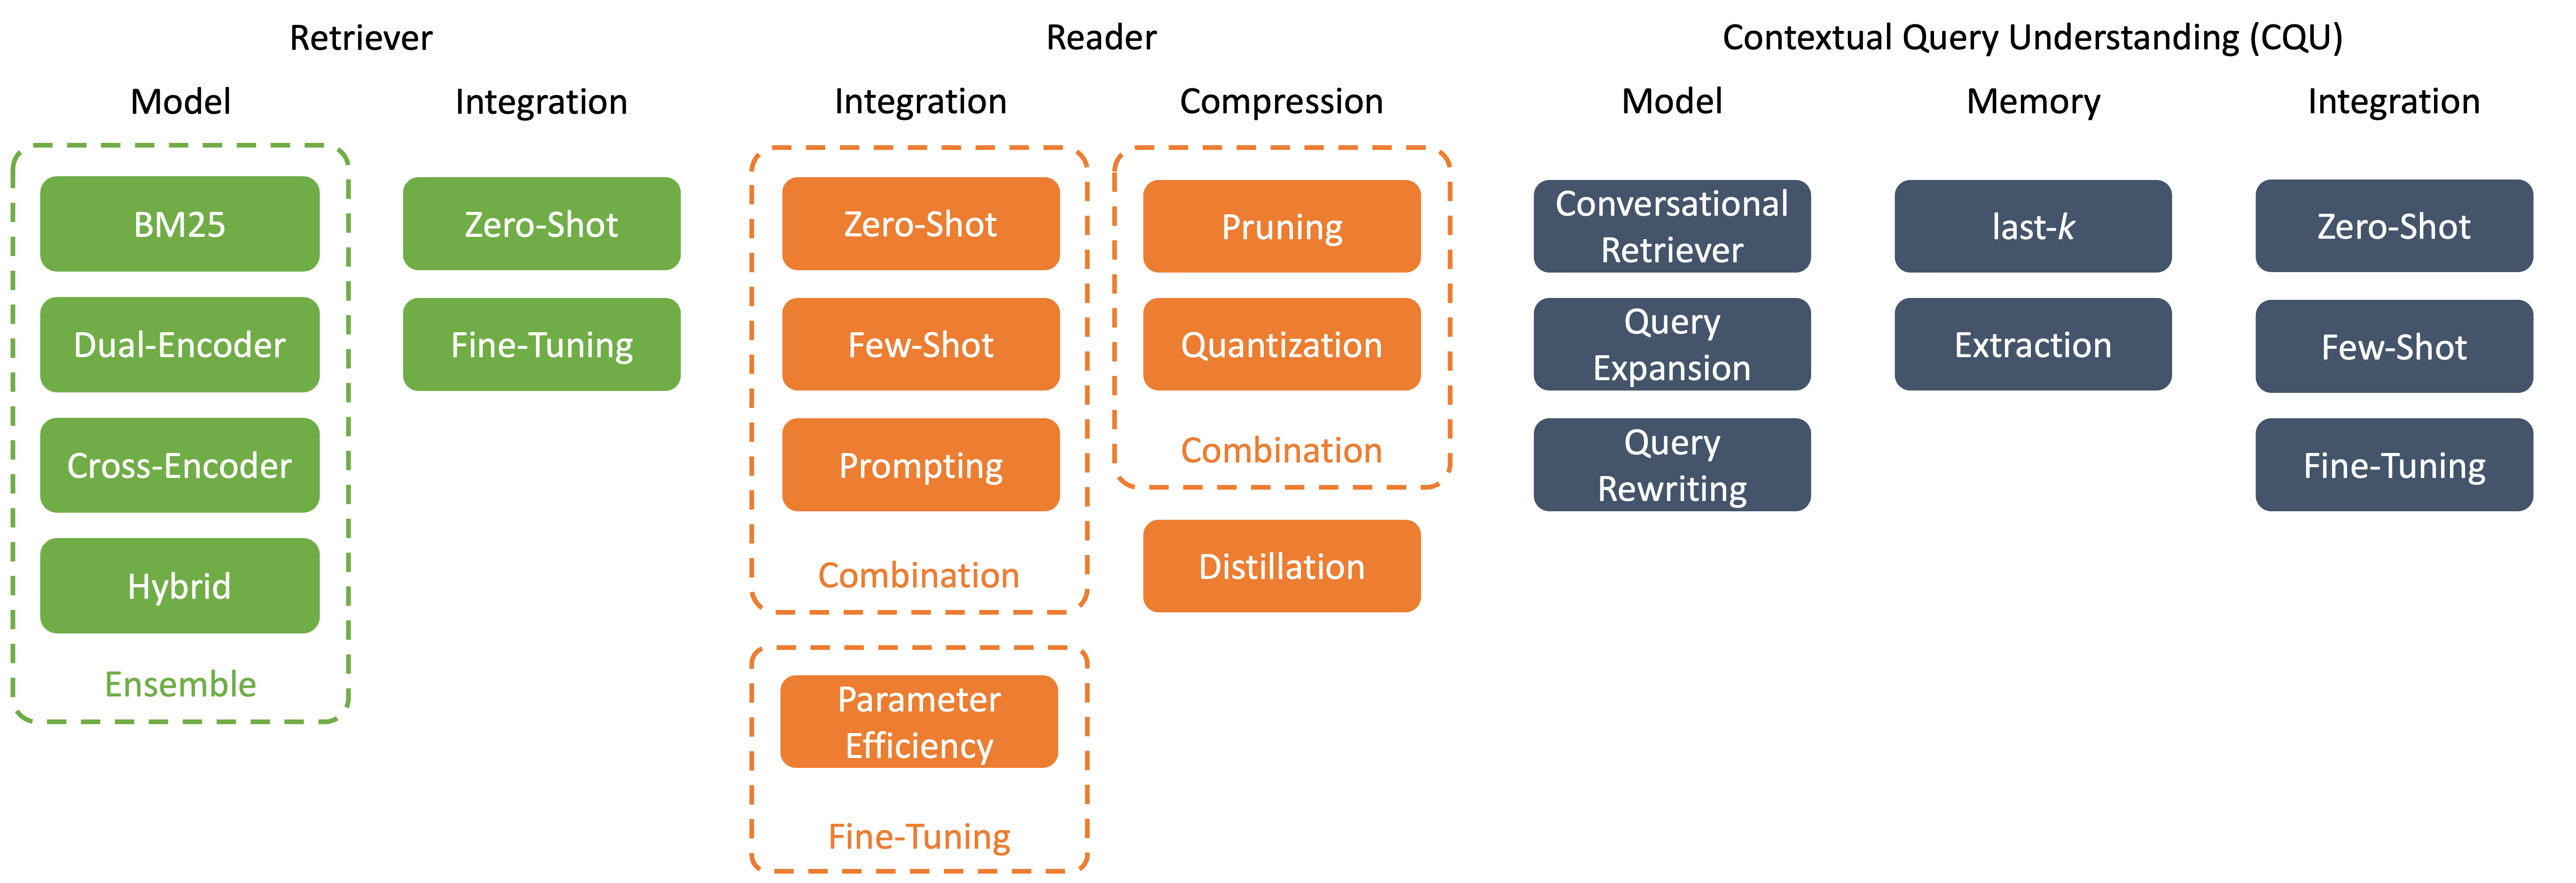
\includegraphics[width=\textwidth]{Grafiken/all_components_conrag.png}
    \caption{All Components of the System Architecture}
    \label{fig:all-components-conrag-grid}
\end{figure}

\subsection{Extraction}
\label{subsec:index}

Figure \ref{fig:extract-pipeline-implementation} illustrates the extraction pipeline implemented for this thesis' \gls{poc}, resulting in the creation of the \textit{document model} of the passages forming the knowledge source. This pipeline comprises the following steps:

\begin{figure}
    \centering
    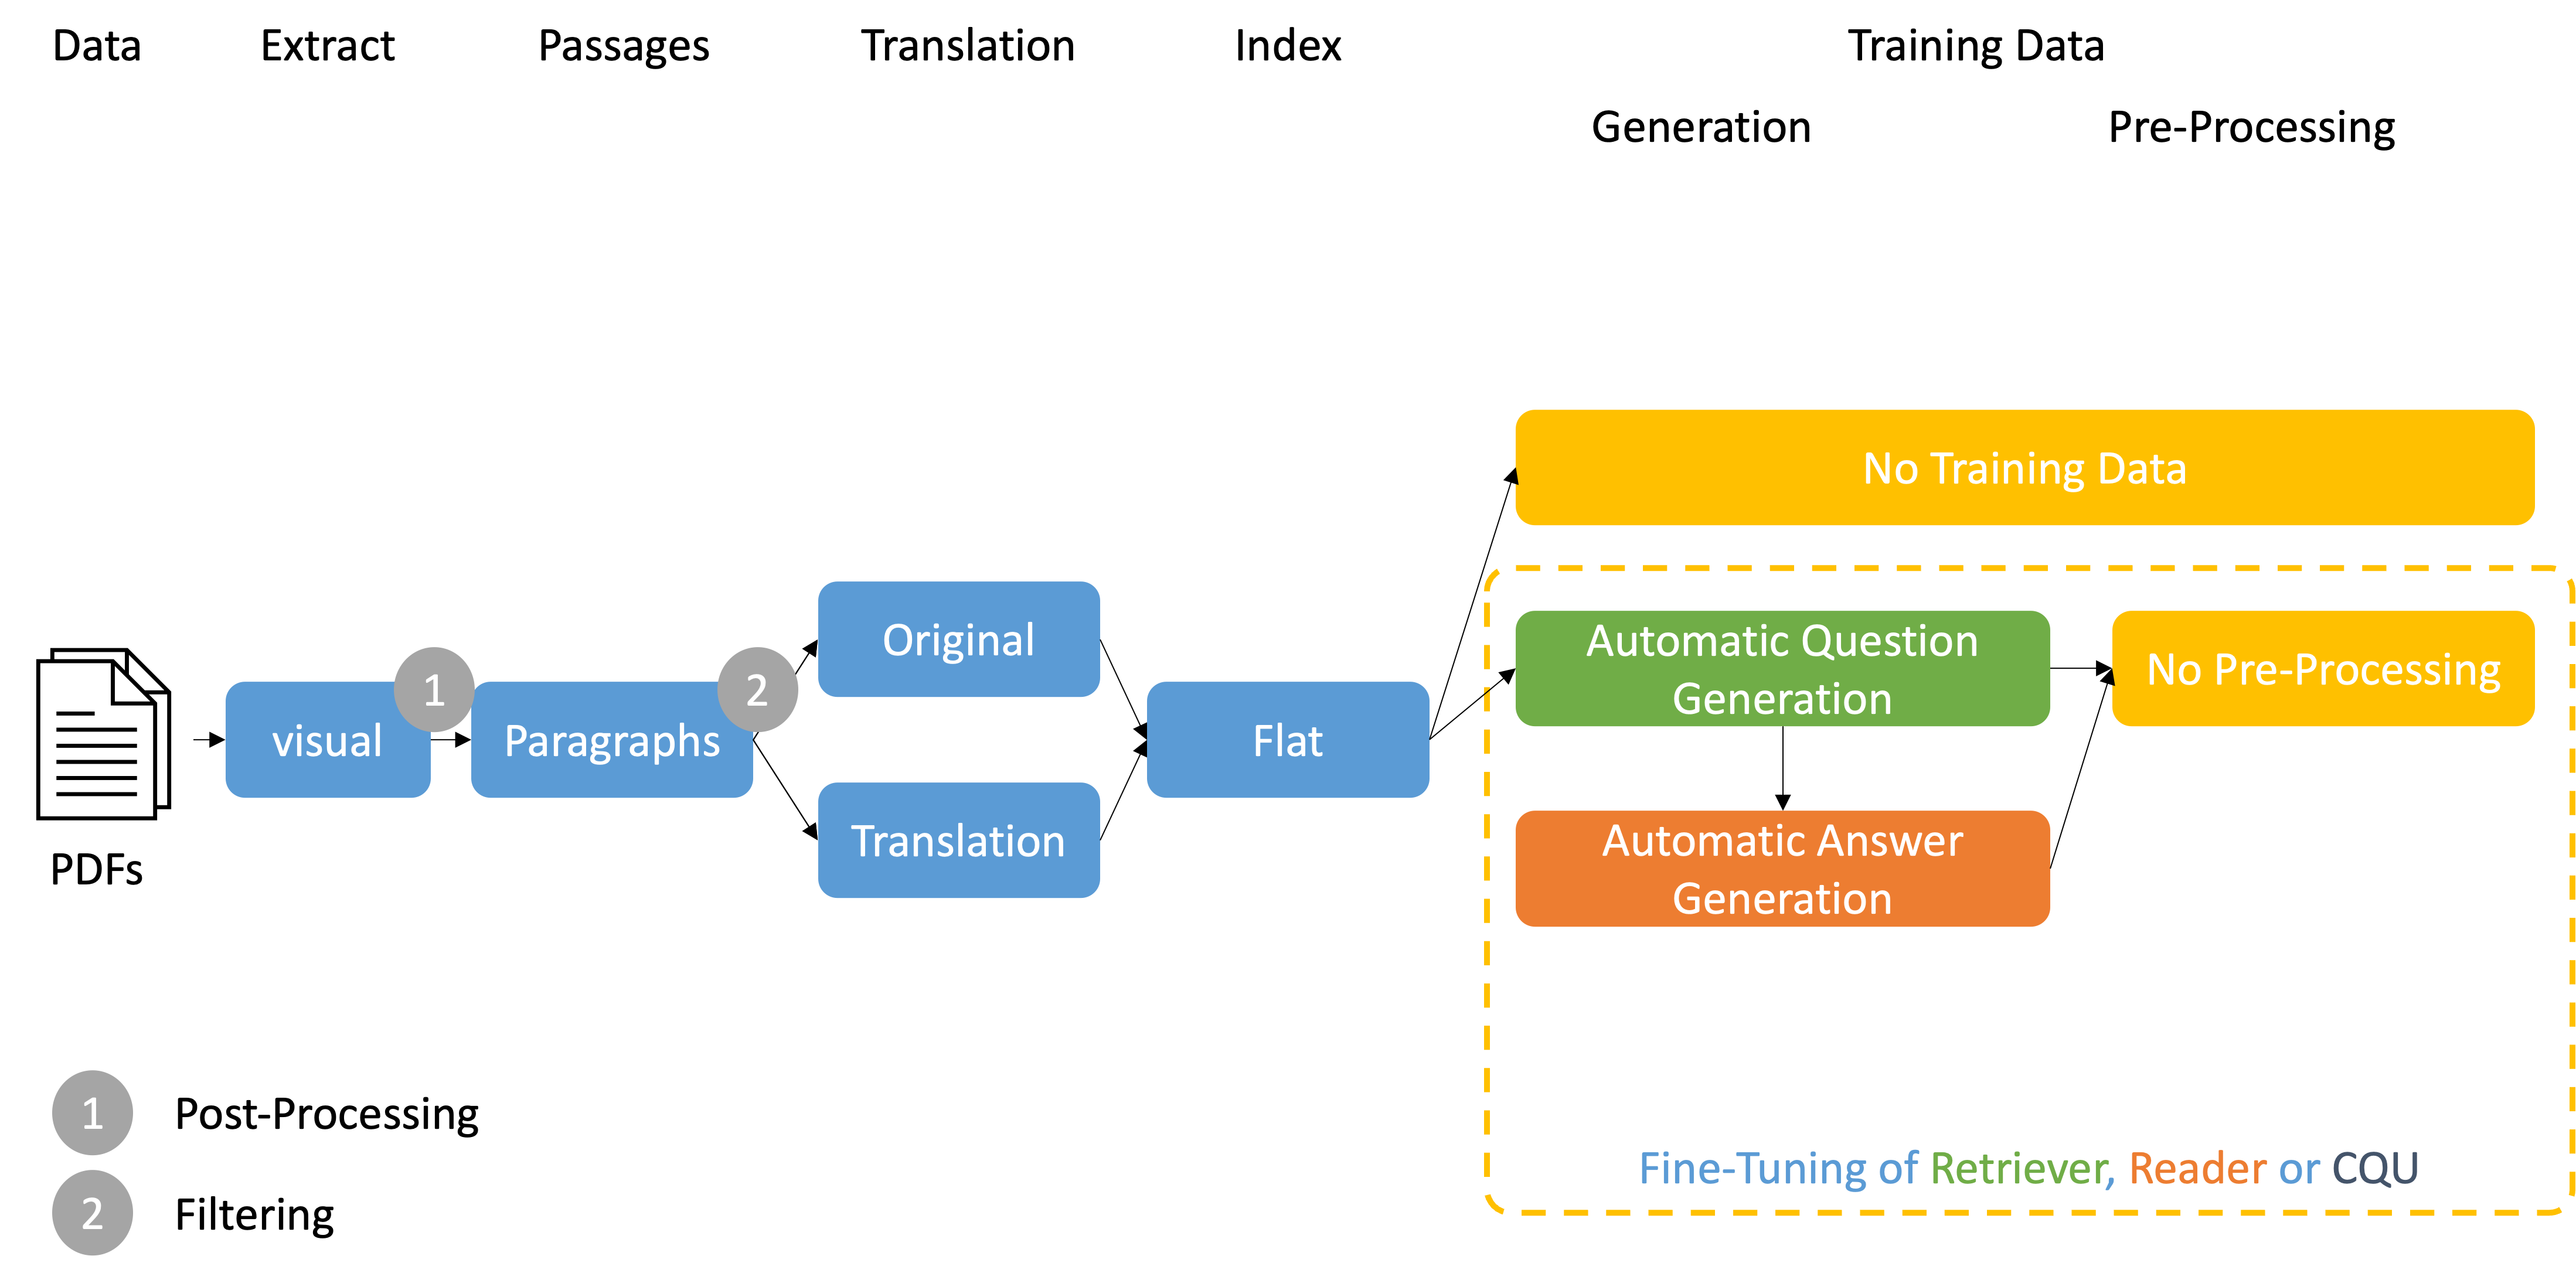
\includegraphics[width=\textwidth]{Grafiken/Evaluation/extract_implemented.png}
    \caption{Implemented Extraction Pipeline}
    \label{fig:extract-pipeline-implementation}
\end{figure}

\begin{enumerate}
    \item \textit{Extract:} Visual extraction using the Google Cloud Vision API for PDF OCR\footnote{\url{https://cloud.google.com/vision/docs/pdf}}, followed by post-processing.
    \item \textit{Passages:} Extraction of paragraphs using the NLTK tokenizer-based Text Splitter by Langchain\footnote{\url{https://python.langchain.com/docs/modules/data\_connection/document\_transformers/text\_splitters/split\_by\_token\#nltk}}, followed by filtering.
    \item \textit{Translation:} Retaining the original data and providing translations from German to English and English to German using the Google Cloud Translation API\footnote{\url{https://cloud.google.com/translate/docs/overview}}.
    \item \textit{Index:} A flat index, with each passage extended to include the title of the document.
    \item \textit{Training Data:} Application of Automatic Question Generation, Automatic Answer Generation, and Automatic Conversation Generation using the Llama2-7b-chat and LeoLama-7b models quantized using GPTQ.
\end{enumerate}

\textbf{Extraction Pipeline:} In step (1), when given a PDF, the textual content of every page is extracted as plain text using OCR without paragraph awareness. This choice was made after simple qualitative experiments, which revealed that using direct methods leads to an unclean text corpus for the given PDFs. In the OCR, line breaks are detected and inserted as characters like \texttt{\textbackslash n}. The textual content of separate pages is concatenated using a linebreak character \texttt{\textbackslash n}. For post-processing, all \texttt{\textbackslash n} characters will be replaced by spaces \texttt{" "}. This process results in a fully concatenated text corpus for every PDF.

In step (2), the NLTK-based Text Splitter receives a text corpus and identifies sentences in a first step based on punctuation. This list of sentences is then combined recursively to ensure it does not exceed the desired maximum length of 240 tokens. This choice of token length was made based on reference works and their chosen token lengths (see Section \ref{sec:related_work}). It's also important to consider the input token sizes of the later-implemented Reader components. If an identified sentence itself has more than 240 tokens, e.g., 400, it will still be kept as a 400-token-long passage. Misidentifying sentences can occur quickly, e.g. text originally corresponding to a table, which cannot be easily split into sentences:

\begin{quote}
    \texttt{Coding reference Appendix 1: Semester 1 30 CPS A03-16-3 Semester 2 30 CP Semester 3 30 CPS Key qualifications: Patient Orientation, Consultation, Moderation / Presentation, English, Interdisciplinary Collaboration 4 CP 2 CP 4 CP Scientific Writing 1 Thematic Area I: Scientific Principles and Methods Scientific Writing ...}
\end{quote}

To ensure that passages do not exceed a maximum character length, identified passages will be truncated at the next empty space after reaching 1300 characters. For comparison and to understand the impact of this filtering on the knowledge source, Figure \ref{fig:er-german-passage-length-old} displays the distribution of passage lengths before filtering, compared to the distribution after filtering in Figure \ref{fig:er-german-passage-length}, which illustrates the influence of filtering. The filtering process removes outliers at 1300 characters, a decision that aligns with the later components of the system.

\begin{figure}
    \centering
    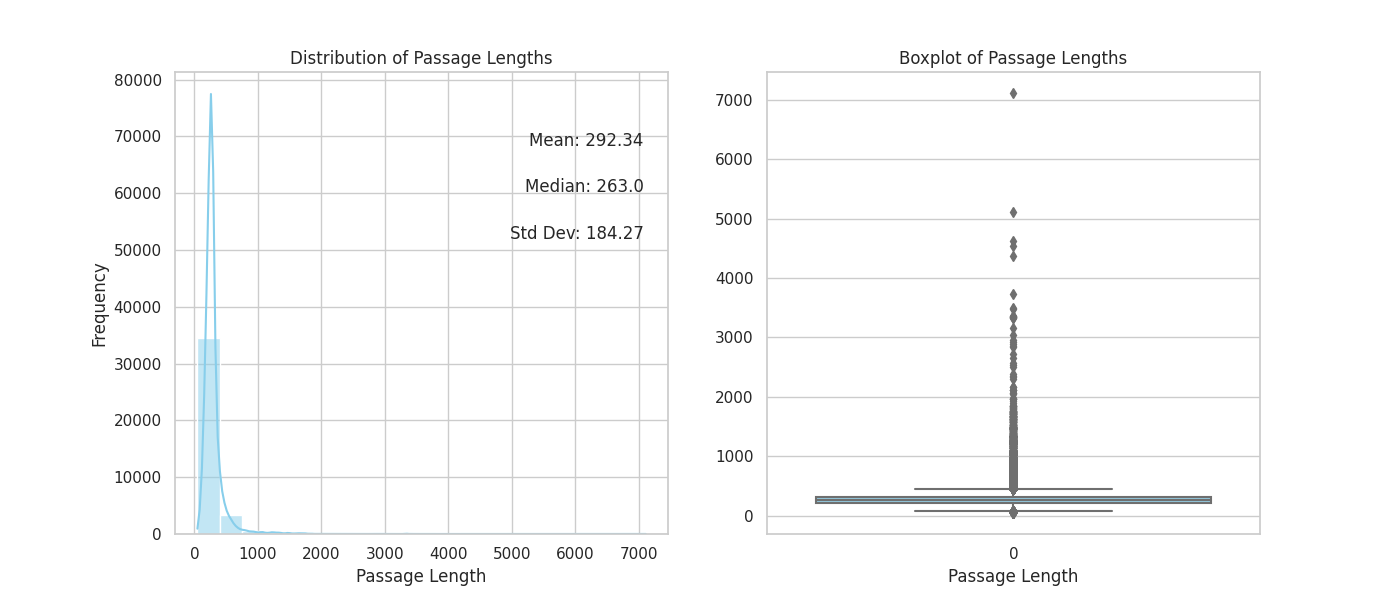
\includegraphics[width=\textwidth]{Grafiken/Statistiken/IndexGerman_Passage_Length_Statistics_old.png}
    \caption{Passage Length Distribution of the German \gls{er} Dataset before Filtering}
    \label{fig:er-german-passage-length-old}
\end{figure}

In Step (3), every passage and all in Step (5) generated questions of the German and English \gls{er} dataset are translated using the Google Translate API. This creates a two more dataset in addition to the existing two, which are directly based on the document's language.

The final Step (4) toward the \textit{knowledge source} is the index creation. To simplify the later \gls{rag} system, the decision was made not to use a hierarchical index structure. However, this could lead to problems when users need to find specific information within one document and want to perform metadata-filtering. To address this, all passages have the title of the document from which they were extracted concatenated to them in the following way:

\begin{quotation}
    \{passage\} + \texttt{ - } + \{documentName\}
\end{quotation}

This approach enables the retriever and reader to identify passages and their corresponding documents in a single step, as opposed to hierarchical index implementations that necessitate multiple steps and potentially multiple databases for embeddings and metadata of the passages. This method has been chosen because, in this use-case, the only utilized and easy extractable metadata of a document is a documents title (e.g., \textit{Examination Regulation for the Master Data and Computer Science}, with some even including the date). Other use-cases may require more complicated appraoches. For the translated datasets, the document name will be translated, as described in Step (3).

\textbf{Data Augmentation:} Step (5) of the extraction pipeline involves data augmentation. For \textit{Question Generation} based on a given passage, the few-shot approach from \textit{PROMPTAGATOR} \cite{dai_promptagator_2022} has been employed. For the English \gls{er} dataset, the following prompt is used to generate a question, given a passage and $i$ examples:

\begin{quote}
   \texttt{System Prompt:}\\
    \texttt{You are an assistant generating one question given a context. Please start your generated question with the indicator 'Generated Question:' Here are some examples:} \\
   \{i\}\texttt{-Example:} \\
   \texttt{Context:} \{passage\} \\
    \texttt{Generated Question:} \{question\} \\ \\
    \texttt{User:} \\
    \texttt{Generate the question based on the following context:}\\
    \{passage\}
\end{quote}

The snippet in the System Prompt is looped four times to accommodate the number of examples. The examples represent different question types, which themeself indicate different answer types, in order to add some variety to the generated data. The used examples can be found in the appendix \ref{ref:appendixA-data-augmentation-few-shot-prompt}. The Prompt is generally designed to be used with a chat fine-tuned model, as it showed better results in a qualitative evaluation. For English question generation, the \textit{Llama2-7B-Chat-GPTQ}\footnote{\url{https://huggingface.co/TheBloke/Llama-2-7b-Chat-GPTQ}} is employed. It's a quantized version of the original Llama2-7B-Chat Model by Meta \cite{touvron_llama_2023}. For the German \gls{er}, the same prompt translated to English is used. For the German tasks, the \textit{Leo-Hessianai-7B-Chat-GPTQ}\footnote{\url{https://huggingface.co/TheBloke/leo-hessianai-7B-chat-GPTQ}} model is used, which is a quantized version of a German language fine-tuned Llama2-7B-Chat Model \cite{pluster_leolm_2023}.

It's worth noting that the English Llama2-7B-Chat was capable of directly understanding the system prompt and generating questions with the indicator \texttt{Generated Question}, which made using the generated text easier. However, the German \gls{llm} struggled with this Few-Shot task and often generated multiple responses that didn't start with the indicator \texttt{Generierte Frage}. Additionally, the model sometimes included answers after the questions. To extract the single question from the generated text in the German \gls{llm} output, the text is cropped after a \texttt{:} and \texttt{?}, so the string enclosed by these characters is used as the question for a given passage. 

The choice of Llama2-based models was based on their new state-of-the-art results in multiple benchmarks, as demonstrated by these models in the open-source \gls{llm} niche \cite{touvron_llama_2023}. Additionally, the work of Plüster et al. \cite{pluster_leolm_2023} on LeoLama opens the opportunity to compare the performance of German and English \gls{llm}s from the same family.

For \textit{Answer Generation} the previously generated questions per passage are being used. In order to provide high quality answers, the choice was made to use gpt-3.5-turbo

\subsection{Retriever}
\label{subsec:retriever-impl}

The implemented retrievers can be found in Figure \ref{fig:retriever-implementation}. Given the limited availability of (synthetic) data suitable for fine-tuning, the decision was made to exclusively utilize top-performing \gls{ood} zero-shot retrievers. Fine-tuning a model on such a small dataset could lead to a high risk of overfitting. To assess retriever performance, the synthetic dataset will be used for benchmarking. Among the top-performing retrievers from the BEIR benchmarks, the following three retrievers have been choosen:

\begin{enumerate}
    \item \textbf{BM25:} This employs the standard lexical-based best match algorithm with hyperparameters $k_1=1.5$, $b=0.75$, and $\epsilon=0.25$. It is implemented using the open-source project \textit{rank-bm25} \footnote{\url{https://github.com/dorianbrown/rank_bm25}}.
    \item \textbf{BM25 + CE:} This uses a BM25 retriever in combination with a Cross-Encoder re-ranker, which serves as the baseline established in BEIR \cite{thakur_beir_2021}. This combination continues to perform as the state-of-the-art. The Cross-Encoder utilized is the same as the one in the BEIR baseline implementation: \textit{ms-marco-MiniLM-L-6-v2} \cite{wang_minilm_2020}, specifically the implementation provided on Hugging Face \footnote{\url{https://huggingface.co/cross-encoder/ms-marco-MiniLM-L-6-v2}}. For German indices, a German version of \textit{ms-marco-MiniLM-L-6} is used: \textit{ms-marco-MiniLM-L-6-en-de-v1} \footnote{\url{https://huggingface.co/cross-encoder/msmarco-MiniLM-L6-en-de-v1}}.
    \item \textbf{Large DPR:} For the large \gls{dpr}, the embedding model from OpenAI, \textit{text-embedding-ada-002} \footnote{\url{https://platform.openai.com/docs/models/embeddings}}, is employed. The parameter size of this model is estimated to be around 350 million parameters\cite{muennighoff_sgpt_2022}\footnote{As OpenAI does not publicly provide information on their model specs, there exists only estimates}.
\end{enumerate}

These retrievers have been implemented and evaluated based on the synthetic data, and the results are presented in Section \ref{sec:results}.

\begin{figure}
    \centering
    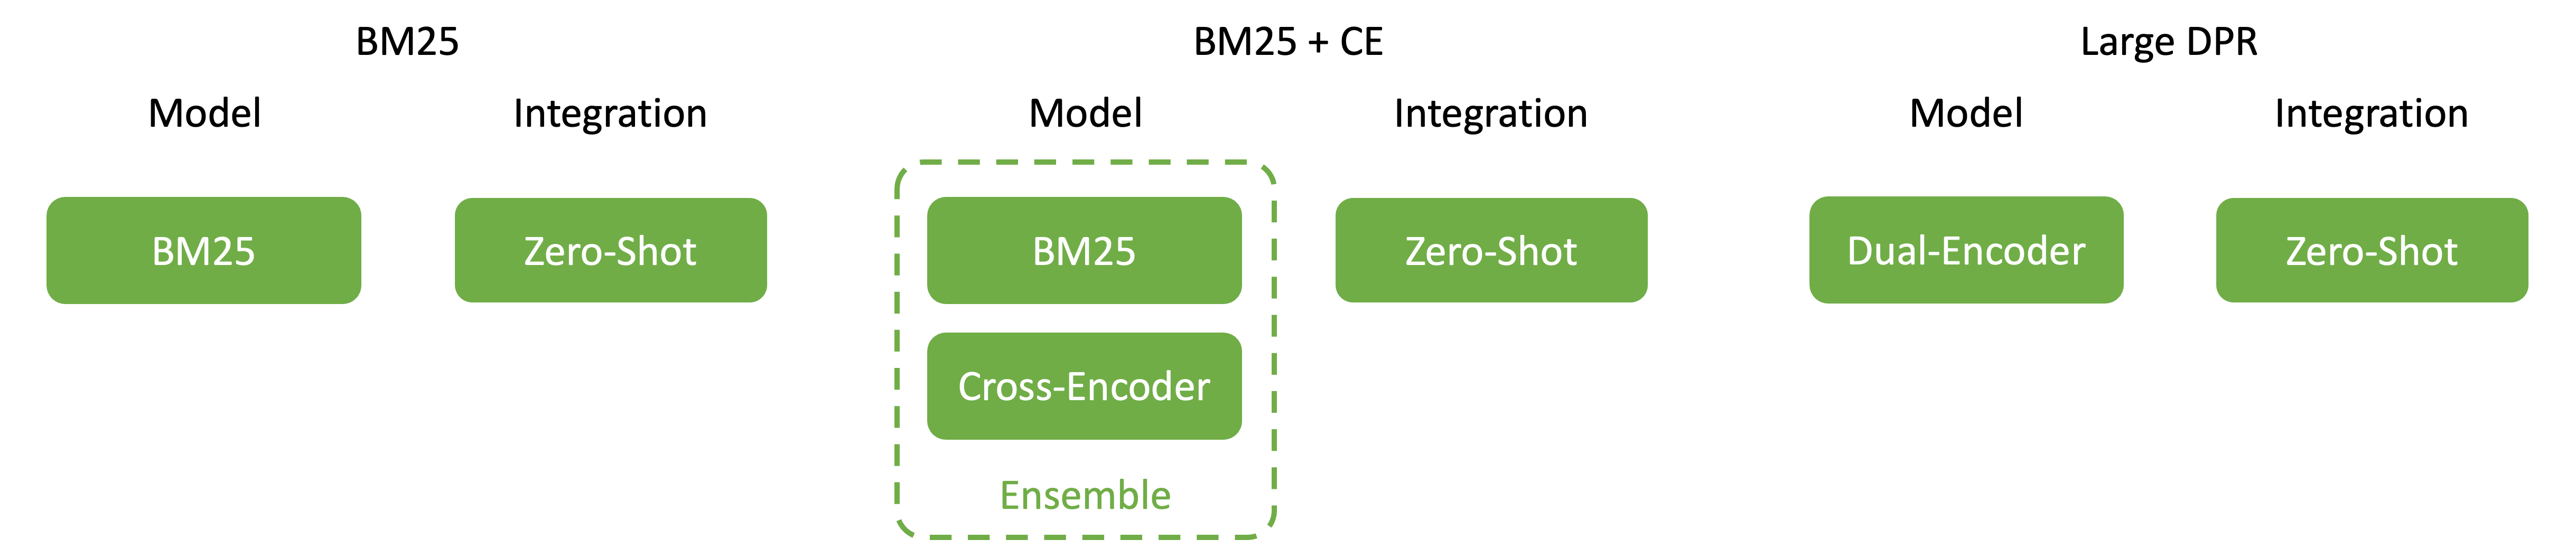
\includegraphics[width=\textwidth]{Grafiken/Evaluation/retriever_implemented.png}    
    \caption{Implemented Retrievers}
    \label{fig:retriever-implementation}
\end{figure}

\subsection{Reader}
\label{subsec:reader-impl}

The implemented readers can be found in Figure \ref{fig:reader-implementation}. Due to the limited hardware resources and high-quality data, the decision was made to only use zero-shot pre-trained \glspl{llm}s for the reader component and not fine-tune any. The following readers have been chosen:

\begin{enumerate}
    \item \textbf{gpt-3.5-turbo:} GPT 3.5 Turbo is part of the OpenAI chat completion family\footnote{\url{https://platform.openai.com/docs/models/gpt-3-5}}. Details on the parameters are not available. However, the latest published research by OpenAI indicates 175B parameters for the model on which GPT 3.5 Turbo was built. In general, the model is an \gls{llm} trained using human feedback on chat-like completion tasks \cite{ouyang_training_2022}. It accepts up to 4,096 tokens as input.
    \item \textbf{Llama2-7B-Chat-GPTQ:} This is a quantized version of the original Llama2-7B-Chat Model by Meta \cite{touvron_llama_2023}. The model is an \gls{llm} trained on chat-instruction datasets \cite{ouyang_training_2022}. The model is available on Hugging Face\footnote{\url{https://huggingface.co/TheBloke/Llama-2-7b-Chat-GPTQ}}. The model is quantized using GPTQ \cite{muennighoff_sgpt_2022}. However, the provider did not report any benchmarks indicating the accuracy drop of the GPTQ version compared to the original. It accepts up to 4,096 tokens as input.
    \item \textbf{leo-hessianai-7B-chat-GPTQ:} \textit{Linguistisch Erweitertes Offenes Language Model} (LeoLM) is a German tasks fine-tuned version of the original Llama2-7B-Chat model. The original Llama2 is fine-tuned on a large corpus of German language texts, and multiple adjustments are applied to overcome the problem of forgetting. This results in a maximum input token length of 8,000 tokens. In addition to original German chat instruction-based datasets, automatic translated English benchmark datasets are used as well. Benchmarking results indicate an increase in German language capabilities while maintaining English language task performance \cite{pluster_leolm_nodate}.
\end{enumerate}

Generally, \textbf{gpt-3.5-turbo} acts as a higher-end benchmark. It is a state-of-the-art \gls{llm} with high popularity in the media and developer community. \textbf{Llama2-7B-Chat-GPTQ} should be a hardware resource-efficient alternative pre-trained model, especially the quantized version that can run on consumer hardware. \textbf{leo-hessianai-7B-chat-GPTQ} is representative of a German native model, providing further insights into language dependencies and the performance of \gls{llm}s, as the use case involves multiple indices in German and English.

Further approaches such as evaluating different fine-tuning approaches have been excluded, as they would open a huge problem field itself and can't be covered in an appropriate manner in this thesis. Therefore this thesis rather focuses on a holistic \gls{poc} to show and evaluate one possible implementation approach of the in Section \ref{chap:main} introduced framework using the mentioned \gls{llm}s.

\begin{figure}
    \centering
    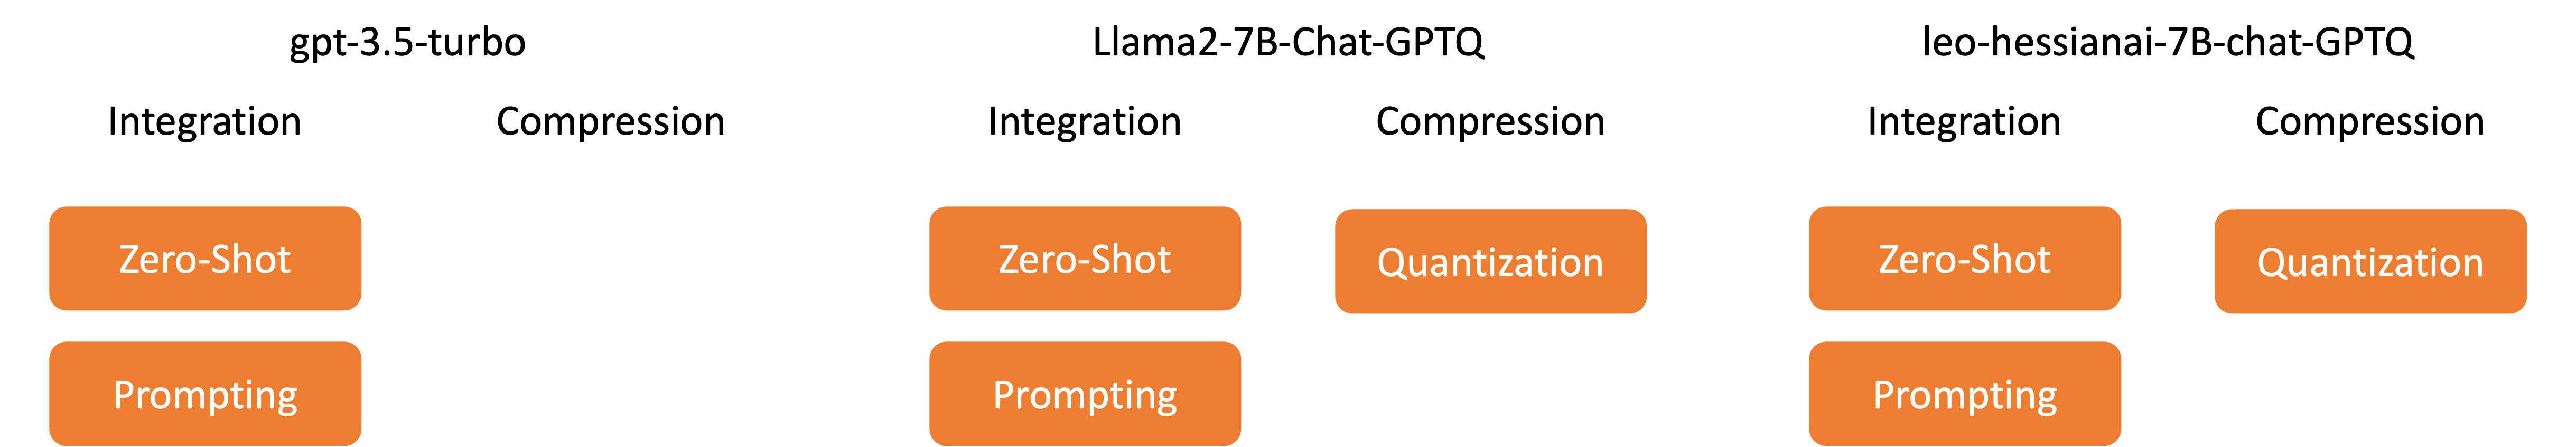
\includegraphics[width=\textwidth]{Grafiken/Evaluation/reader_implemented.png}
    \caption{Implemented Readers}
    \label{fig:reader-implementation}
\end{figure}

\subsection{CQU}
\label{subsec:cqu-impl}

\section{Experimental Results}
\label{sec:results}

\subsection{Data Augmentation Quality}
\label{subsec:data-augmentation-quality}

\subsection{Retrieval Results}
\label{subsec:retrieval-results}

\subsection{Reader Results}
\label{subsec:reader-results}

\subsection{Conversational Question Answering Results}
\label{subsec:convqa-results}